% 1977 q2 trough folded from sheet
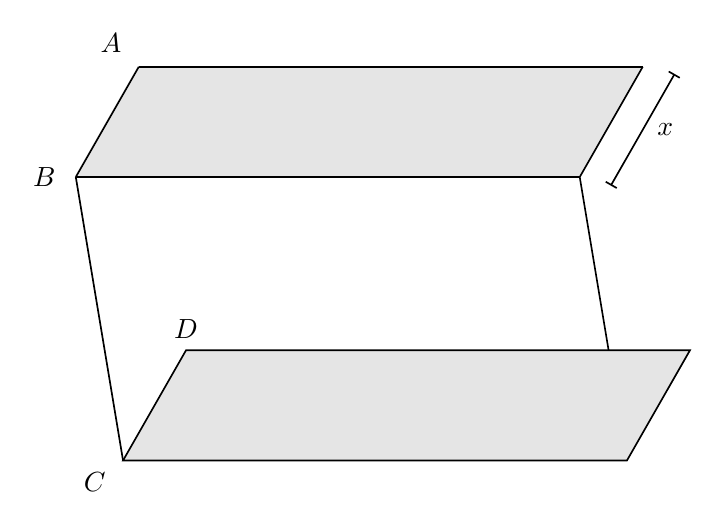
\begin{tikzpicture}[x=1cm,y=1cm,font=\normalsize,line width=.6pt,
  geom/.style={solid,line width=.6pt},
  lbl/.style={font=\normalsize,inner sep=2pt}]
% top flap parallelogram
\coordinate (T1) at (0,2.6);
\coordinate (T2) at (6.4,2.6);
\coordinate (T3) at (5.6,1.2);
\coordinate (T4) at (-0.8,1.2);
% bottom flap
\coordinate (U1) at (0.6,-1.0);
\coordinate (U2) at (7.0,-1.0);
\coordinate (U3) at (6.2,-2.4);
\coordinate (U4) at (-0.2,-2.4);
\fill[gray!20] (T1)--(T2)--(T3)--(T4)--cycle;
\fill[gray!20] (U1)--(U2)--(U3)--(U4)--cycle;
% middle bottom edge line
\draw[geom] (T4)--(T3);
\draw[geom] (T1)--(T2);
\draw[geom] (T1)--(T4);
\draw[geom] (T2)--(T3);
\draw[geom] (T4)--(U4);
\coordinate (V) at (5.9666666667,-1.0);
\draw[geom] (T3)--(V);
\draw[geom] (U4)--(U3)--(U2)--(U1)--cycle;
% labels
\node[lbl,above left,xshift=-4pt,yshift=3pt] at (T1) {$A$};
\node[lbl,left,xshift=-5pt] at (T4) {$B$};
\node[lbl,below left,xshift=-4pt,yshift=-2pt] at (U4) {$C$};
\node[lbl,above,yshift=2pt] at (U1) {$D$};
% x measures the flap width, parallel to AB.
\draw[geom] (6.8,2.5)--(6,1.1);
\draw[geom] (6.73,2.54)--(6.87,2.46);
\draw[geom] (5.93,1.14)--(6.07,1.06);
\node[lbl,right=3pt] at (6.4,1.8) {$x$};
\end{tikzpicture}
